\documentclass[pdflatex,sn-mathphys-num]{sn-jnl}% Math and Physical Sciences Numbered

\usepackage{graphicx}%
\usepackage{multirow}%
\usepackage{amsmath,amssymb,amsfonts}%
\usepackage{amsthm}%
\usepackage{mathrsfs}%
\usepackage[title]{appendix}%
\usepackage{xcolor}%
\usepackage{textcomp}%
\usepackage{manyfoot}%
\usepackage{booktabs}%
\usepackage{multicol}
\usepackage{fancyvrb}
\usepackage{geometry}
\usepackage{titlesec}
\usepackage{xcolor}
\usepackage{parskip}
\usepackage{array}
\usepackage{multirow}
\usepackage{booktabs}
% Commented out biblatex because sn-jnl class loads natbib (incompatible)
% If you need bibliographies, use natbib commands: \citep{}, \citet{}, \bibliography{}
% \usepackage[backend=biber,style=apa]{biblatex}
% \addbibresource{references.bib}

\usepackage{hyperref}
\usepackage{xurl}             % Permite que los \url{} largos hagan salto de línea en cualquier caracter (evita overfull hbox en la sección de Referencias)
\usepackage{fontawesome5} % For the GitHub icon
\usepackage[justification=centering]{caption}
\usepackage[linesnumbered,ruled,vlined]{algorithm2e}
\setlength{\topmargin}{-0.4in}
\setlength{\textheight}{9in}
\usepackage{comment}
\usepackage{listings}%
% In your preamble:
\usepackage{enumitem} % For custom list formatting
\newlist{questions}{enumerate}{1}
\setlist[questions,1]{
  label=\textbf{Q\arabic*:}, % Label format "Q1:", "Q2:", ...
  leftmargin=2em,           % Indent spacing
  itemsep=1em               % Space between questions
}



%%%%



\raggedbottom



% Code Packages

\usepackage{listings}
\usepackage{xcolor}

\definecolor{headerbackground}{rgb}{1, 1, 1}
\definecolor{rulecolor}{rgb}{0.7, 0.7, 0.7}

% Define C keywords including standard library functions
\lstdefinestyle{algorithmstyle}{
  backgroundcolor=\color{white},
  basicstyle=\ttfamily\scriptsize,
  keywordstyle=\bfseries, % Bold for keywords
  commentstyle=\itshape, % Italic for comments
  stringstyle=,
  numberstyle=\tiny,
  numbers=left,
  numbersep=10pt,
  breaklines=true,
  frame=trbl,
  framerule=0.8pt,
  rulecolor=\color{rulecolor},
  framesep=5pt,
  xleftmargin=15pt,
  xrightmargin=5pt,
  language=C, % This is crucial
  tabsize=2,
  showstringspaces=false,
  alsoletter={\_},
  morekeywords={printf, scanf, malloc, free, sizeof, puts, gets}, % Add standard library functions
}

% ============================================ %
% Configuración adicional agregada para el      %
% reporte de CAN Bus (protocolo CAN)            %
% ============================================ %
\usepackage{siunitx}          % Unidades (Mbit/s, ns, V, etc.)
\sisetup{per-mode=symbol}
\usepackage{tabularx}         % Columnas que ajustan su ancho al \linewidth (evita tablas desbordadas)
\usepackage{ragged2e}         % \RaggedRight dentro de columnas X (mejor que justificado forzado)
\newcolumntype{Y}{>{\RaggedRight\arraybackslash}X}

% Resaltado rápido de bits dominantes/recesivos dentro del texto
\newcommand{\dominant}{\textbf{dominante (0)}}
\newcommand{\recessive}{\textbf{recesivo (1)}}

\newcommand{\codeheader}[1]{%
  \noindent%
  \fcolorbox{rulecolor}{headerbackground}{%
    \makebox[\dimexpr\linewidth-2\fboxsep-2\fboxrule][l]{%
      \textbf{Code:} \ttfamily{#1}%
    }%
  }%
  \vspace{-0.5\baselineskip}
}

\begin{document}

\title[Article Title]{RF-Car}

\author*[1,2]{\fnm{Contreras R} \sur{Orlando}}\email{\{al348390,al464376\}@edu.uaa.mx}

\affil[3]{\orgdiv{Department of Electronic Systems}, \orgname{UAA}, \orgaddress{\street{Av. Universidad 940}, \city{Aguascalientes}, \postcode{20131}, \state{Aguascalientes}, \country{México}}}

%%==================================%%
%% Sample for unstructured abstract %%
%%==================================%%

\abstract{}

\keywords{CAN Bus, ISO 11898, Bus de campo, Arbitraje, STM32, Comunicación serial, CAN FD.}

\maketitle

\section{Introducción}\label{sec1}

\newpage
\section{Sistema Mínimo}
\subsection{STM32F103C8T6 - BluePill}
\subsection{TB6612FNG - Puente H}
The TB6612FNG driver was used to control the vehicle's motors, as it allows for the management of two DC motors with speed and direction control. Here is shown the block diagram and pinout of the TB6612FNG:
\begin{figure}[h]
    \centering
    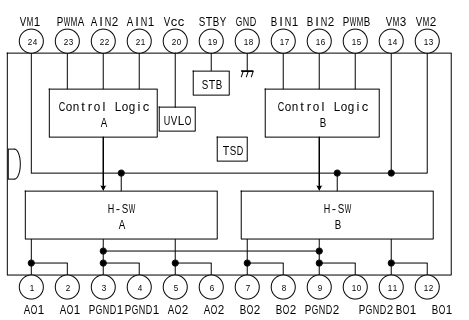
\includegraphics[width=0.8\textwidth]{src/Driver_Pinout.png}
    \caption{Pinout del Driver TB6612FNG.}
    \label{fig:Driver_Pinout}
\end{figure}

Additionaly, the functions of each pin of the TB6612FNG are integrated, as shown in Table \ref{fig:Driver_Pinout_List}.


\begin{figure}[h]
    \centering
    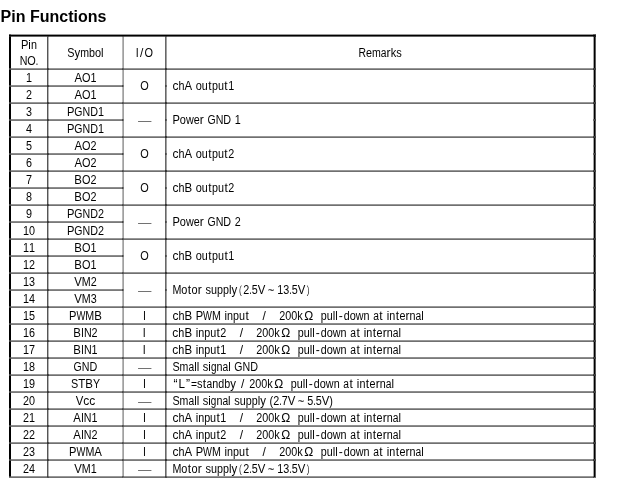
\includegraphics[width=0.65\textwidth]{src/Driver_Pinout_List.png}
    \caption{Tabla de funciones de cada Pin del Driver TB6612FNG.}
    \label{fig:Driver_Pinout_List}
\end{figure}
\newpage
The typical application circuit of the TB6612FNG is shown in Figure \ref{fig:Driver_Circuit}.
\begin{figure}[h]
    \centering
    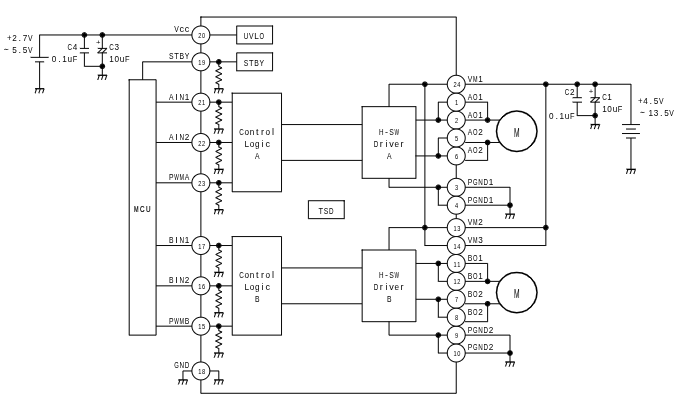
\includegraphics[width=0.8\textwidth]{src/Driver_Diagram.png}
    \caption{Typical Application Circuit of the TB6612FNG.}
    \label{fig:Driver_Circuit}
\end{figure}

We could see that the typical application circuit of the TB6612FNG is very simple, and it can be easily integrated into our project. By researching about the TB6612FNG Implementations, we found that the capacitor of 10 uF on VCC is not necessary, and it can be removed from the circuit. We could see that on the SparkFun breakout board, the capacitor of 10 uF is not present, as shown in Figure \ref{fig:Driver_SparkFun}. 
%\cite{SparkFunTB6612FNG}


\begin{figure}[h]
    \centering
    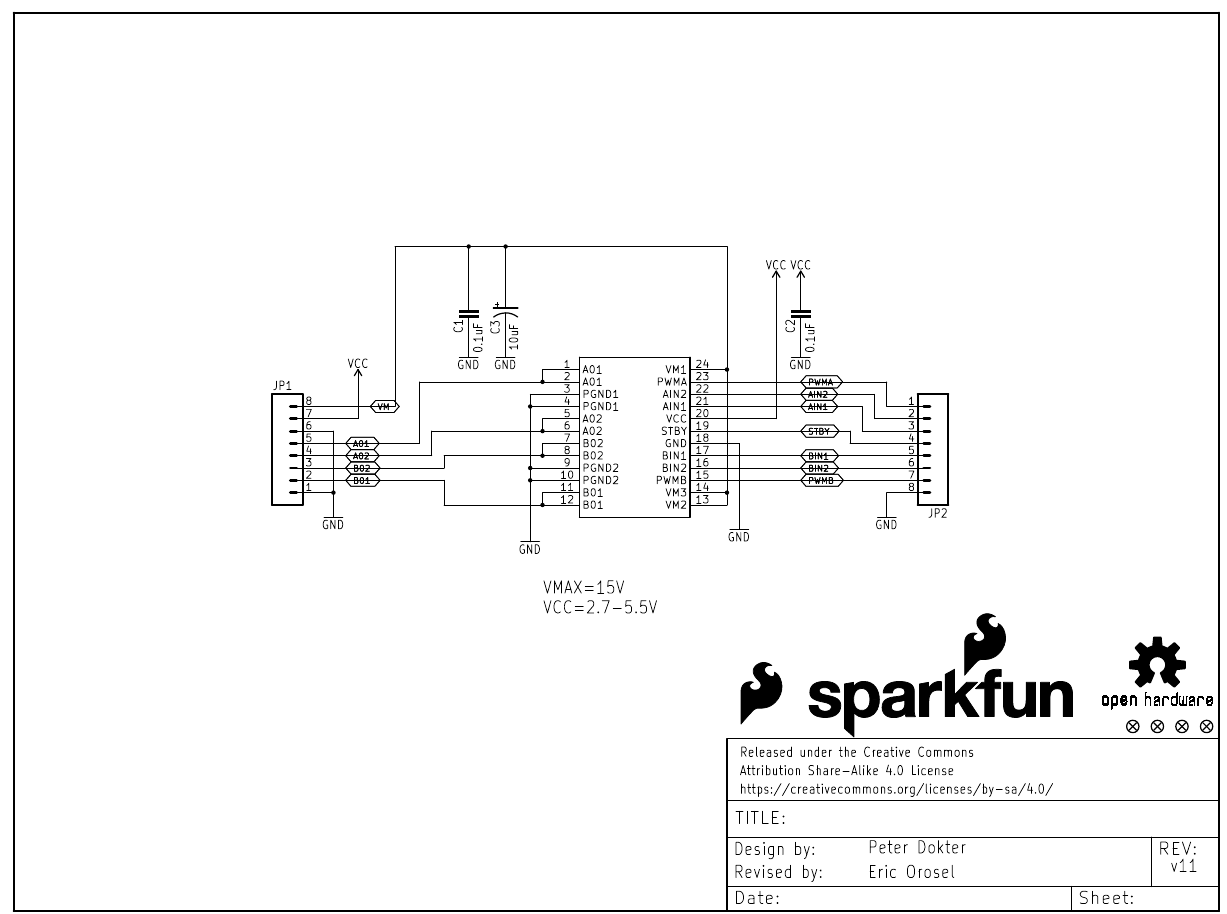
\includegraphics[width=1\textwidth]{src/Driver_SparkFun.png}
    \caption{SparkFun breakout board of the TB6612FNG.}
    \label{fig:Driver_SparkFun}
\end{figure}

%https://github.com/sparkfun/Motor_Driver-Dual_TB6612FNG


\newpage
The device uses two separate supplies:
\begin{itemize}
  \item \textbf{$V_{CC}$}: logic supply, \SIrange{2.7}{5.5}{\volt}.
  \item \textbf{$V_M$}: motor supply, up to \SI{15}{\volt}.
\end{itemize}
 
Keeping both domains separate lets the microcontroller logic run from its own
regulated rail while the motors are fed from a battery or power supply.
Because the two rails have very different current profiles, each one needs its
own decoupling, as discussed next.
 
\subsection{Decoupling Capacitors}
 
The typical application circuit in the datasheet places a \SI{0.1}{\micro\farad}
and a \SI{10}{\micro\farad} capacitor on both $V_M$ and $V_{CC}$. Each value
has a different purpose.
 
\paragraph{Role of each rail.}
The $V_{CC}$ rail only feeds the control logic, so its current demand is a few
milliamps and mostly constant. The $V_M$ rail feeds the H-bridge output stage,
which draws sharp current pulses at the PWM frequency and receives back-EMF
spikes from the motor when the bridge switches or brakes. Capacitance on $V_M$
is therefore the more critical of the two. Compact breakout boards often
reduce the number of capacitors compared with the reference circuit, leaving
extra bulk capacitance to the user.
\paragraph{Capacitor value and frequency.}
A real capacitor behaves as a series $RLC$ network \ref{fig:ESR}: the capacitance $C$, the
equivalent series resistance (ESR) and the equivalent series inductance (ESL).
%https://jlcpcb.com/blog/capacitor-esr-explained

\begin{figure}[h]
    \centering
    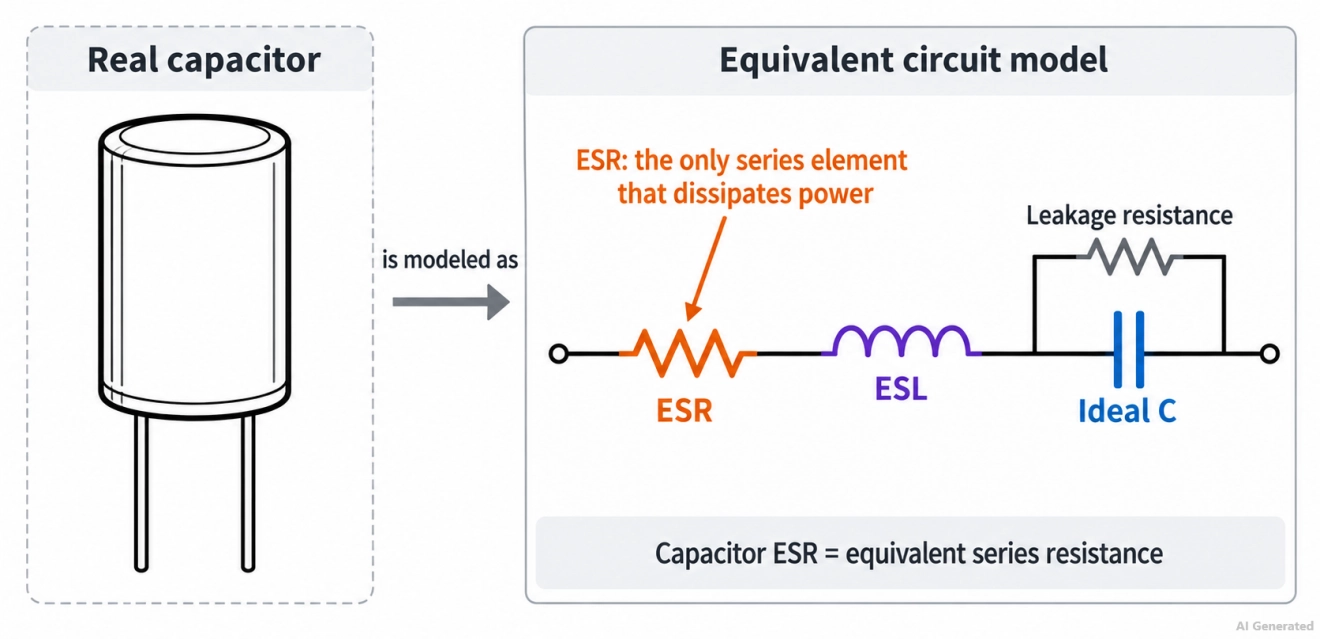
\includegraphics[width=0.6\textwidth]{src/ESR.png}
    \caption{Equivalent series resistance (ESR) and inductance (ESL) of a real capacitor.}
    \label{fig:ESR}
\end{figure}
Its impedance is
$$
Z(f) = \mathrm{ESR} + jw(\mathrm{ESL}) + \frac{1}{jw C} = \mathrm{ESR} + j\left( 2\pi f \,\mathrm{ESL} - \frac{1}{2\pi f C} \right),
$$
\begin{equation}
  Z(f) = \mathrm{ESR} + j\left( 2\pi f \,\mathrm{ESL} - \frac{1}{2\pi f C} \right).
\label{eq:Impedance}
\end{equation}
Given the self-resonant frequency $f_{SRF}$ is where the inductive and capacitive \textbf{reactances} cancel each other, the capacitor behaves as a capacitor below $f_{SRF}$ and as an inductor above it. So we could take the equation \ref{eq:Impedance} to find the self-resonant frequency of a capacitor, which is given by:
$$
\text{Im}(Z)=\text{Im}( \mathrm{ESR} + j\left( 2\pi f \,\mathrm{ESL} - \frac{1}{2\pi f C} \right)) =0 \Rightarrow 2\pi f \,\mathrm{ESL} - \frac{1}{2\pi f C} = 0
$$

Below the self-resonant frequency
\begin{equation}
  f_{SRF} = \frac{1}{2\pi\sqrt{\mathrm{ESL}\cdot C}}
\end{equation}
the capacitor acts as a capacitor; above it, the ESL dominates and it behaves
as an inductor, which makes it useless for filtering. This is why two
capacitors are used in parallel: the large one covers low frequencies and the
small one covers high frequencies.
 
\begin{figure}[h]
    \centering
    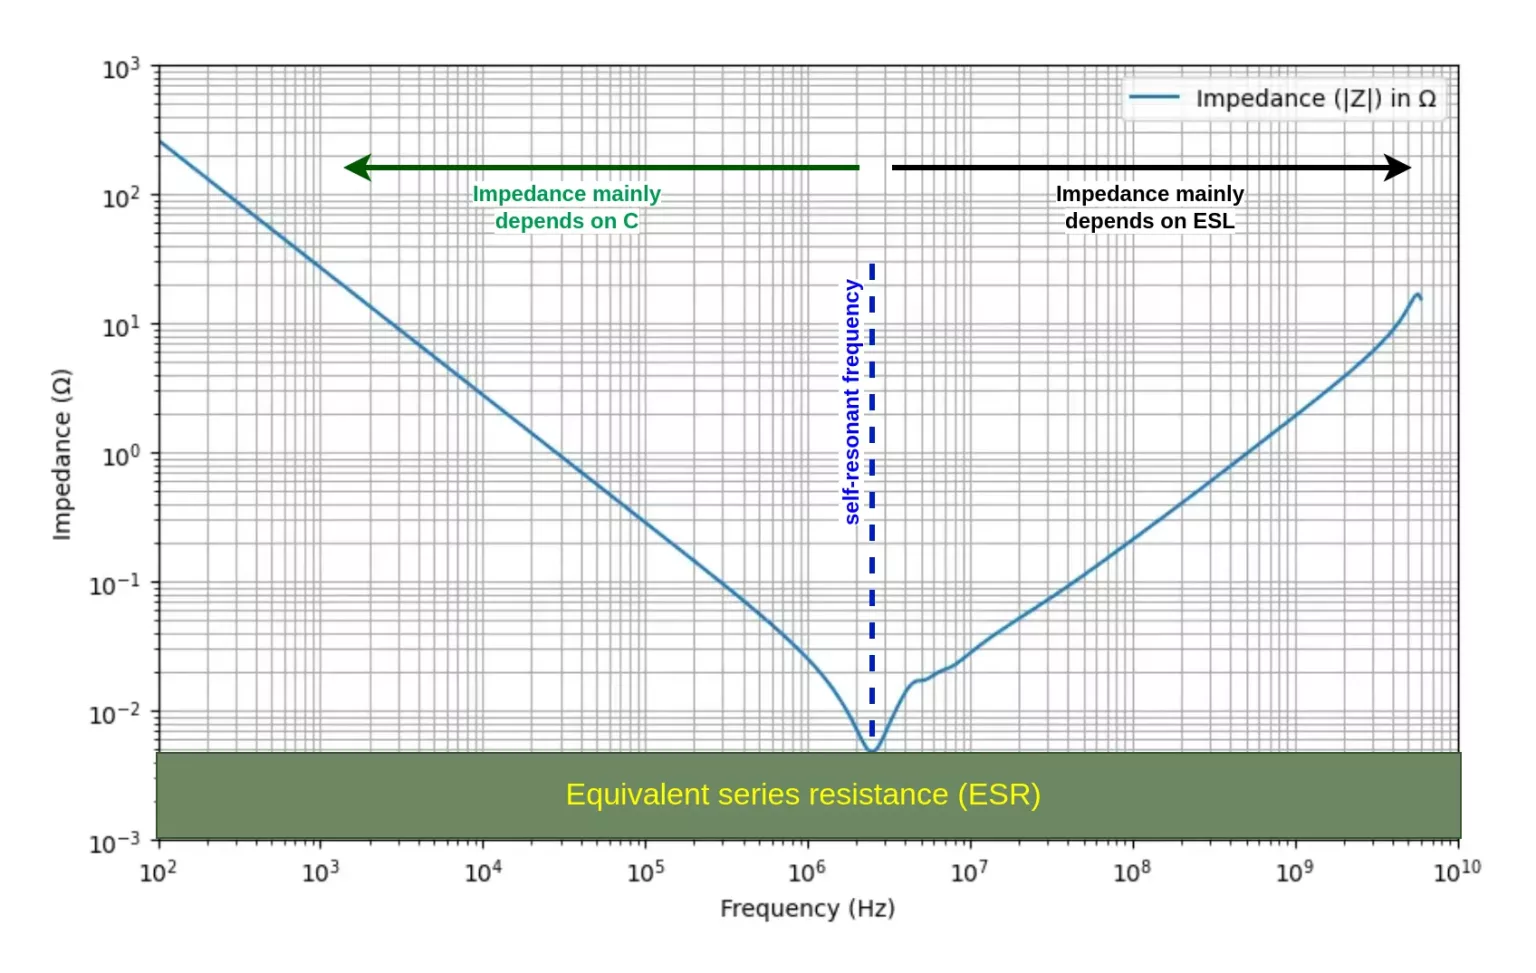
\includegraphics[width=0.8\textwidth]{src/ESR_ESL.png}
    \caption{Impedance of a real capacitor, showing the effect of ESR and ESL.}
    \label{fig:ESR_ESL}
\end{figure}
%https://thecapacitorhub.com/2024/03/02/esr-of-a-capacitor-and-its-effects-on-impedance/
The ideal reactance $X_C = 1/(2\pi f C)$ at two frequencies of interest is:
\begin{table}[h]
  \centering
  \caption{Ideal capacitive reactance of the two decoupling values.}
  \begin{tabular}{lcc}
    \toprule
    $C$ & $X_C$ at \SI{100}{\kilo\hertz} & $X_C$ at \SI{10}{\mega\hertz} \\
    \midrule
    \SI{10}{\micro\farad}  & \SI{0.16}{\ohm} & \SI{1.6}{\milli\ohm} \\
    \SI{0.1}{\micro\farad} & \SI{15.9}{\ohm} & \SI{0.16}{\ohm} \\
    \bottomrule
  \end{tabular}
\end{table}
 
At the PWM frequency (up to \SI{100}{\kilo\hertz}) the \SI{10}{\micro\farad}
capacitor provides the low impedance path. At the tens of megahertz present in
the switching edges, only the \SI{0.1}{\micro\farad} capacitor remains
effective, since its smaller ESL pushes its resonance much higher.
 
\paragraph{Capacitor size and voltage ripple.}
The bulk capacitor supplies the current pulse of the bridge while the source
cannot respond. A first-order estimate of the voltage droop on $V_M$ is
\begin{equation}
  \Delta V \approx \frac{I \,\Delta t}{C},
  \label{eq:VoltageRipple}
\end{equation}
where $I$ is the pulse current and $\Delta t$ its duration. 

For example, with a 1A pulse lasting 5 us (half a period at 100 kHz) given capacitor values of 10 uF and 100 uF, the voltage droop is:
$$
\Delta V = \frac{1 \text{ A} \cdot 5 \times 10^{-6} \text{ s}}{10 \times 10^{-6} \text{ F}} = 0.5 \text{ V}  \quad
\Delta V = \frac{1 \text{ A} \cdot 5 \times 10^{-6} \text{ s}}{100 \times 10^{-6} \text{ F}} = 0.05 \text{ V}
$$
Ten times less with \SI{100}{\micro\farad}. This is a worst-case estimate, since the
supply also contributes current. Larger $C$ reduces ripple, but increases the
inrush current at power-up and the board area.
 

\paragraph{Package size (0402, 0603, 0805).}
Surface-mount ceramic capacitors are named by their size code. In the
imperial system, the codes correspond to the following dimensions (the metric code of the same part is different, e.g.\ imperial 0402 is metric 1005):
\begin{table}[h]
  \centering
  \caption{Common imperial package sizes for ceramic capacitors.}
  \begin{tabular}{lccl}
    \toprule
    Imperial code & Size (mm) & Typical ESL & Typical use here \\
    \midrule
    0402 & $1.0 \times 0.5$ & about \SIrange{0.4}{0.7}{\nano\henry} & \SI{0.1}{\micro\farad}, high-frequency bypass \\
    0603 & $1.6 \times 0.8$ & about \SIrange{0.6}{0.9}{\nano\henry} & \SI{0.1}{\micro\farad} to \SI{1}{\micro\farad}, general purpose \\
    0805 & $2.0 \times 1.25$ & about \SIrange{0.8}{1.2}{\nano\henry} & \SI{1}{\micro\farad} to \SI{10}{\micro\farad}, bulk \\
    \bottomrule
  \end{tabular}
\end{table}
\begin{figure}[h]
    \centering
    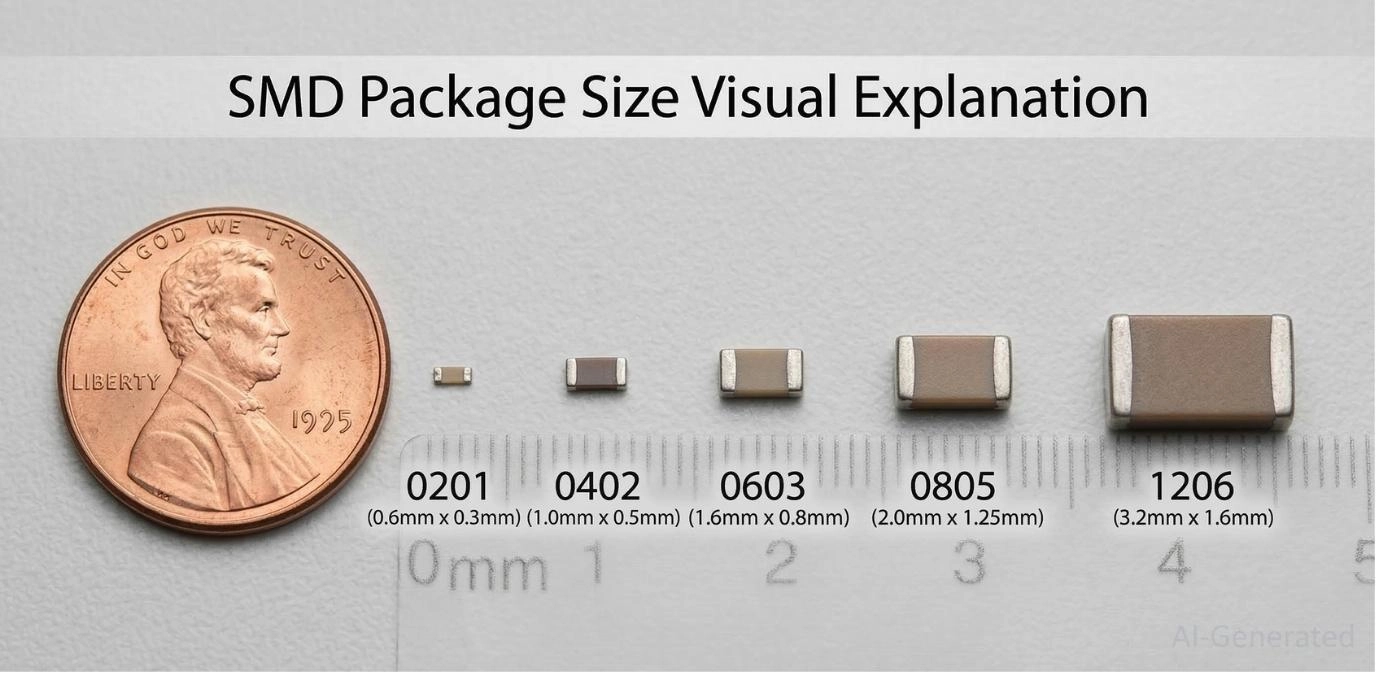
\includegraphics[width=0.8\textwidth]{src/SMD_Sizes.png}
    \caption{SMD package sizes for ceramic capacitors.}
    \label{fig:SMD_Sizes}
\end{figure}
 
The package affects the capacitor in three ways:
\begin{itemize}
  \item \textbf{ESL.} A smaller body has a shorter current path, so its ESL is
        slightly lower and its self-resonant frequency slightly higher. In
        practice the difference is small, and the inductance of the PCB
        traces and vias to the capacitor is usually larger than the ESL of
        the part itself, so placement matters more than the package.
  \item \textbf{Capacitance and voltage available.} A given package can only
        hold a limited capacitance at a given voltage rating. A
        \SI{0.1}{\micro\farad} capacitor is easy in 0402 or 0603, while
        \SI{10}{\micro\farad} in ceramic generally needs 0805 or larger for a
        voltage rating suitable for $V_M$.
  \item \textbf{DC bias derating.} For the same value and voltage rating, a
        smaller package loses more of its capacitance when the DC voltage
        increases, and this is more severe in X5R/X7R dielectrics. A
        \SI{10}{\micro\farad} 0603 part rated at \SI{10}{\volt} can drop to a
        fraction of its nominal value at \SI{5}{\volt} bias, so the effective
        capacitance should be checked in the manufacturer's curves.
\end{itemize}
Larger packages are also more susceptible to cracking from board flex, which
is a consideration for boards that are handled or mounted on vibrating
platforms such as robots.


\paragraph{Ceramic versus electrolytic.}
\begin{table}[h]
  \centering
  \caption{Typical characteristics of the two capacitor types.}
  \begin{tabular}{lll}
    \toprule
    & Ceramic (MLCC) & Aluminum electrolytic \\
    \midrule
    Typical value here & \SI{0.1}{\micro\farad} (up to \SI{10}{\micro\farad}) & \SI{10}{\micro\farad} and above \\
    ESR & Very low & Higher \\
    ESL & Very low (about \SI{1}{\nano\henry}) & Higher (order of \SI{10}{\nano\henry}) \\
    Self-resonance & Tens of MHz (for \SI{0.1}{\micro\farad}) & Hundreds of kHz \\
    Polarity & Non-polarized & Polarized \\
    Main use & High-frequency noise & Bulk energy, low-frequency ripple \\
    Caveat & Capacitance drops with DC bias (X5R/X7R) & Aging; voltage rating must be respected \\
    \bottomrule
  \end{tabular}
\end{table}
 
With these typical values, a \SI{0.1}{\micro\farad} ceramic with \SI{1}{\nano\henry}
of ESL resonates near \SI{16}{\mega\hertz}, while a \SI{10}{\micro\farad}
electrolytic with \SI{10}{\nano\henry} resonates near \SI{500}{\kilo\hertz}.
The actual values depend on the package and manufacturer and should be taken
from the capacitor datasheet.

 
\paragraph{Practical recommendations.}
\begin{itemize}
  \item Use 0402 or 0603 for the \SI{0.1}{\micro\farad} ceramic and place it
        as close as possible to the
        $V_{CC}$ and $V_M$ pins, with short traces to ground.
  \item On $V_M$, add a bulk capacitor of \SI{10}{\micro\farad} or more. If the
        motor supply is far from the board or the motors draw high current,
        use \SIrange{47}{100}{\micro\farad}. Equation \ref{eq:VoltageRipple} can be used to estimate the voltage droop.
  \item Choose a voltage rating well above the maximum $V_M$; for a
        \SI{15}{\volt} maximum, a \SI{25}{\volt} part is a common choice.
\end{itemize}
 
We conclude then the next values for the decoupling capacitors:

\begin{table}[h]
  \centering
  \caption{Selected decoupling capacitors for the TB6612FNG.}
  \begin{tabular}{llllll}
    \toprule
    Rail & Value & Type & Size & Voltage & Target frequency \\
    \midrule
    $V_{CC}$ & \SI{0.1}{\micro\farad} & Ceramic X7R & 0603 (or 0402) & \SI{50}{\volt} & \SI{1}{\mega\hertz} to tens of \si{\mega\hertz} \\
    $V_M$ & \SI{0.1}{\micro\farad} & Ceramic X7R & 0603 (or 0402) & \SI{50}{\volt} & \SI{1}{\mega\hertz} to tens of \si{\mega\hertz} \\
    $V_M$ & \SI{22}{\micro\farad} & Tantalum & 1210 & \SI{16}{\volt} & DC to about \SI{1}{\mega\hertz} (PWM up to \SI{100}{\kilo\hertz}) \\    \bottomrule
  \end{tabular}
\end{table}

\begin{comment}
    Resources
    https://honda-tech.com/forums/tech-misc-15/any-information-honda-can-bus-2825633/
    https://github.com/marcellatwin/honda-canbus-project
    https://www.cjindustriesaustralia.com/blogs/canbus-settings/honda-canbus-settings-cr-v-fit-jazz-civic-odyssey-accord-city-etc?srsltid=AfmBOooJQAEVHB_3T1qvhvghN4wXMAKU_n9l7jSUo22kCEmljVZEn51B
    https://forum.autosportlabs.com/viewtopic.php?t=6148
    https://arxiv.org/html/2408.09265v1
    https://github.com/commaai/opendbc/blob/master/README.md#how-to-port-a-car
\end{comment}
\section{Conclusión}\label{sec:conclusion}
El protocolo CAN se ha consolidado durante casi cuatro décadas como el bus de comunicación de referencia en sistemas embebidos distribuidos, gracias a un diseño elegante que resuelve de forma determinista el acceso múltiple al medio mediante arbitraje bit a bit, y a un sistema de detección de errores excepcionalmente robusto para el bajo costo de su capa física. Si bien su ancho de banda y tamaño de carga útil resultan limitados frente a las demandas actuales de los vehículos autónomos y conectados, su evolución hacia CAN FD -y en desarrollo, CAN XL- demuestra la vigencia del enfoque original. Para el trabajo práctico con microcontroladores STM32, el periférico bxCAN/FDCAN ofrece una vía directa y bien soportada por HAL para integrar nodos CAN en proyectos de instrumentación, robótica o redes de sensores distribuidos.

\end{document}